\documentclass[oneside,11pt,french,table]{book}
\usepackage[french]{babel}
\usepackage[margin=1in]{geometry}

% Lorem ipsum paragraphs
\usepackage{lipsum}
\usepackage{bm}
% Paragraph spacing
\usepackage{parskip}

% Custom fonts. This package is only available with XeLaTex (pdflatex is a mess to deal with)
\usepackage{fontspec}
\setmainfont{GeneralSans}[
    Path = assets/fonts/,
    Extension = .otf,
    UprightFont = *-Regular,
    ItalicFont = *-Italic,
    BoldFont = *-Bold,
    BoldItalicFont = *-BoldItalic
]

% Fancy chapters
\usepackage[Bjornstrup]{fncychap}
\ChTitleVar{\Large\flushright\bfseries}

% Default mathematical packages
\usepackage{amsmath}
\usepackage{amsfonts}

% Theorem styling and environments
\usepackage{amsthm}
\theoremstyle{definition}
\newtheorem{definition}{Définition}[chapter]
\theoremstyle{plain}
\newtheorem{theorem}[definition]{Théorème}
\theoremstyle{remark}
\newtheorem{remark}[definition]{Remarque}

% Boxed theorems
\usepackage{tcolorbox}
\newenvironment{boxdef}{
    \begin{tcolorbox}[boxrule=0pt, frame empty]
    \begin{definition}
}{
    \end{definition}
    \end{tcolorbox}
}

\newenvironment{boxthm}{
    \begin{tcolorbox}[boxrule=0pt, frame empty]
    \begin{theorem}
}{
    \end{theorem}
    \end{tcolorbox}
}

% Graphics
\usepackage{tikz}
\usepackage{float} % for float positioning, in particular the H modifier
\usepackage{subcaption} % for subfigures and subcaptions
\usepackage{pgfplots}
\pgfplotsset{%
  every tick label/.append style = {font=\tiny},
  every axis label/.append style = {font=\scriptsize}
}

% Clickable links
\usepackage{xcolor} % table for colored tables
\definecolor{S4S-light}{HTML}{50527F}
\definecolor{S4S-accent}{HTML}{2C2C5C}
\usepackage[colorlinks,allcolors=S4S-light,linktocpage]{hyperref}

\title{
    Analyse Avancée I \\ \vspace{0.5cm}
    \includegraphics[scale=0.5]{assets/imgs/S4S_logo.png}
}
\author{Students 4 Students}
\date{Septembre 2022}
\begin{document}

\maketitle
\begin{abstract}
    Ces notes sont basées sur les cours des Prof. J. Stubbe et F. Genoud que nous avons eu la chance de suivre à l'EPFL durant nos années académiques, mais également du livre "Elementary Analysis, The Theory of Calculus" de Kenneth A. Ross. En tant qu'étudiants en Physique et Mathématique avancés, nous nous sommes engagés bénévolement à vous donner les meilleurs outils pour débuter votre première année à l'EPFL.  Nous espérons avoir été aussi clairs que possible dans la présentation, afin que vous puissiez vous familiariser sans trop de difficultés avec les premiers et très riches sujets qui font l'objet du cours d'Analyse avancée I.  \\
    
  Nous avons  parfois été volontairement assez succincts dans les démonstrations, pour vous inciter à vous creuser un peu la tête et, si nécessaire, à écrire quelques lignes pour clarifier par vous-même les détails techniques - ou encore à venir en discuter avec nous et vos futurs camarades. Les mathématiques ne s'apprennent pas en lisant, mais en écrivant, c'est ce qu'on vous répétera  sans cesse. \\
  
Nous tenons également à remercier tous nos collègues étudiants avec qui nous travaillons sans relâche et partageons de bons moments.  Nos fortes amitiés se sont forgées dans les amphis de l'EPFL, où nous avons découvert ensemble avec émerveillement les liens profonds entre les mathématiques et la physique mais également profiter ensemble de nos hobbies.\\

Les clés de la réussite ne sont rien d'autre que l'équilibre et la discipline. Trouvez votre mode de vie et ne négligez pas les activités extrascolaires qui vous permettront d'évacuer et de maintenir une bonne santé mentale. La discipline quant à elle vous permettra de persévérer dans les moins bons moments et de toujours maintenir le cap. \\

Enfin, nous sommes infiniment reconnaissants aux professeurs qui, à travers leurs enthousiasmes contagieux et leur vision très large des mathématiques, nous ont finalement amené à vous donner des cours, d'étudiants à étudiants. \paragraph{}
\paragraph{}
Merci à Till Kotitz, Tobia Fjellman, Dylan Samuelian, Roman Paccaud. 
\paragraph{}
\paragraph{}\paragraph{}\paragraph{}\paragraph{}\paragraph{}
Lounès Amziane et Louis Peyratoux 
\end{abstract}

\tableofcontents

\setcounter{chapter}{-1}
\chapter{Introduction Et Motivations}
\section{Les Ensembles Mathématiques $\mathbf{\mathbb{R},\mathbb{Z},\mathbb{N}, \text{ et }  \mathbb{Q}}$}
\subsection{L'ensemble $\mathbb{N}$ des nombres naturels}

On désigne l'ensemble $\{0,1,2,3,...\}$ des nombres entiers non négatifs par $\mathbb{N}$. Cet ensemble est muni de deux opérations :
\begin{itemize}
    \item[$\bullet$] L'addition : $(n,m) \in \mathbb N \times \mathbb N \longrightarrow n + m \in \mathbb N$
    \item[$\bullet$] La multiplication : $(n,m) \in \mathbb N \times \mathbb N \longrightarrow n \cdot m \in \mathbb N$
    \item[]
\end{itemize}
et de la relation d'ordre "plus petit ou égal", dénotée $"\leq"$, qui satisfont les règles de calcul usuelles que vous connaissez déjà. \\

Dans $\mathbb N$, on peut commencer par considérer des équations de la forme
\begin{itemize}
    \item[$\bullet$] $n + x = m$
    \item[$\bullet$] $n \cdot x = m$
\end{itemize}
où $n,m \in \mathbb N$ sont des entiers fixés et $x$ est l'inconnue. 

Certaines de ces équations ont une solution dans $\mathbb N$ : l'équation $3 + x = 7$ possède la solution $x = 4$ et l'équation $2 \cdot x = 10$ possède la solution $x = 5$, mais cela n'est pas le cas de toutes ces équations. Les équations $5 + x = 1$ ou bien $3 \cdot x = 1$ ne sont pas solubles dans $\mathbb N$ et il faut donc agrandir notre ensemble pour traiter ces cas.
\subsection{L'ensemble $\mathbb{Z}$ des nombres relatifs}

On désigne l'ensemble $\{...,-2,-1,0,1,2,...\}$ de tous les nombres entiers par $\mathbb{Z}$. Il est obtenu de $\mathbb N$ en ajoutant tous les éléments inverses pour l'addition. Ainsi, pour tout $n \in \mathbb Z$, il existe un élément $m \in \mathbb Z$, dénoté $-n$, tel que $n + m = 0$. Cette propriété permet de trouver une solution dans $\mathbb Z$ à toutes les équations de la forme
$$n + x = m$$
où $n,m \in \mathbb Z$ sont des entiers fixés. Ces propriétés font de $\mathbb{Z}$ un \textit{anneau} (cf. cours d'algèbre).

\subsection{L'ensemble $\mathbb{Q}$ des nombres rationnels}
On désigne l'ensemble $\displaystyle \{r=\frac{p}{q} : p,q \in \mathbb Z, q \neq 0\}$ de tous les nombres rationnels par $\mathbb{Q}$. Cet ensemble satisfait les mêmes propriétés que $\mathbb Z$ avec l'ajout de l'existence des éléments inverses pour la multiplication. Ainsi, pour tout $q \in \mathbb Q$, il existe un élément $p \in \mathbb{Q}$, dénoté $q^{-1}$ ou $\frac{1}{q}$, tel que $q \cdot p = 1$. Cette propriété permet de trouver une solution dans $\mathbb Q$ à toutes les équations de la forme
$$p \cdot x = q$$
où $p,q \in \mathbb Q$ sont des rationnels fixés. De plus $p$ et $q$ \textbf{sont premiers entre eux}. Toutes ces propriétés font de $\mathbb{Q}$ un \textit{corps} (cf. cours d'algèbre). De plus, $\mathbb{Q}$ satisfait la \textit{propriété Archimédienne} : pour tout rationnel $0 < p < q$, il existe $n \in \mathbb{N}$ tel que $n \cdot p > q$.

On peut donc résoudre les équations du premier degré à coefficients dans $\mathbb Q$, mais qu'en est-il des équations du second degré ? En série d'exercices, vous verrez que l'équation $x^2 = 2$ ne possède pas de solution dans $\mathbb Q$. En d'autres termes, le nombre $\pm \sqrt{2}$ que nous connaissons ne peut pas être rationnel. Cependant, on peut exhiber une suite infinie de nombres rationnels $x_1, x_2, x_3, ...$ qui se rapproche arbitrairement près de $\sqrt{2}$ (voir Figure \ref{fig:seq_sqrt2}). On dit alors que $\mathbb{Q}$ n'est pas \textit{complet}. \\

\begin{figure}[h]
\centering \includegraphics[width = 0.55\textwidth]{./seq_sqrt2.png}
\caption{Suite de rationnels $x_1 = 1$, $x_{n+1} = \frac{1}{2} \left(x_n + \frac{2}{x_n} \right) + \frac{1}{n}$ qui converge vers $\sqrt{2}$ (en rouge)}
\label{fig:seq_sqrt2}
\end{figure}

\subsection{L'ensemble $\mathbb{R}$ des nombres réels}
On désigne l'ensemble de tous les nombres réels (les nombres usuels : $0, \ 1,\  -0.5,\ \pi$, etc ...) par $\mathbb{R}$. \\
Cet ensemble satisfait les mêmes propriétés que $\mathbb{Q}$ et est obtenu à partir de ce dernier en ajoutant les nombres nécessaires (i.e $\pm \sqrt{2}$) pour que l'ensemble soit complet. \\
\\
On notera que $\mathbb{Q}$ est \textit{dense} dans $\mathbb{R}$, c'est-à-dire que pour tout réel $x \in \mathbb R$, pour tout nombre $\varepsilon > 0$, on a $$\{y \in \mathbb R : x - \varepsilon < y < x + \varepsilon\} \cap \mathbb{Q} \neq \emptyset$$
En d'autres termes, tout nombre réel peut être "approché arbitrairement" par des rationnels. \\

\section{Bornes Et Extrema}

Soit $S \subset \mathbb R$ un ensemble de réels. On dit que

\begin{enumerate}
    \item $S$ est \textit{majoré} (ou \textit{borné supérieurement}) s'il existe un nombre $M \in \mathbb R$ tel que pour tout $x \in S$, on ait $x \leq M$. On dit que $M$ est un \textit{majorant} pour $S$.
    \item $S$ est \textit{minoré} (ou \textit{borné inférieurement}) s'il existe un nombre $m \in \mathbb R$ tel que pour tout $x \in S : m \leq x$. On dit que $m$ est un \textit{minorant} pour $S$.
    \item $S$ est \textit{borné} s'il est à la fois majoré et minoré.
\end{enumerate}

Notons que les définitions de majorants et minorants \textbf{ne permettent pas l'unicité} : si $E$ est un ensemble majoré par 0, il est aussi majoré par 0.0001, 2, $5 \pi$ et tout autre nombre réel positif. \\
Dans la plupart des cas, on aimerait savoir quelles sont les "meilleures" bornes d'un ensemble: le majorant le plus petit possible et le minorant le plus grand possible. On les appelle les \textit{extrema} (pluriel de "extremum") de l'ensemble. \\
\paragraph{Définitions - Sup et Inf}
\begin{itemize}
    \item 
Pour $E \subset \mathbb{R}$ un ensemble majoré, on définit son \textit{supremum} comme le plus petit de ses majorants: $$\sup(E) := \min \{ z \in \mathbb{R} : z \geq x \; \forall x \in E \}.$$ 
C'est cette définition qui introduit la notion fondamentale de proximité dans $\mathbb{R}$, centrale à l'analyse. En effet, le supremum vérifie la propriété suivante:
$$\text{ Pour toute quantité } \varepsilon > 0, \text{ on peut trouver un élément } e \in E \text{ tel que } \sup(E) - \varepsilon < e \leq \sup(E).$$
Cela signifie que l'on peut trouver des éléments de $E$ "aussi proches que l'on veut" de son supremum. Si cette propriété n'était pas respectée, il y aurait un $\varepsilon_0 > 0$ pour lequel aucun élément $e \in E$ ne vérifierait $e > \sup(E) - \varepsilon$. Ainsi, par définition, $\sup(E) - \varepsilon$ serait lui-même un majorant de $E$ et contredirait la minimalité de $\sup(E)$. \\
\item
On peut définir de la même manière l'\textit{infimum} de $E$ comme le plus grand de ses minorants: $$\inf(E) = \max \{ z \in \mathbb{R} : z \leq x \, \forall x \in E \}.$$ \\
Par analogie avec le $\sup$, on a la propriété:
$$\text{ Pour toute quantité } \varepsilon > 0, \text{ on peut trouver un élément } e \in E \text{ tel que } \inf(E) \leq e < \inf(E) + \varepsilon.$$
\end{itemize}
\paragraph{}
Ces notions sont mal définies dans $\mathbb{Q}$: prenons par exemple l'ensemble $E = \{ x \in \mathbb{Q} : x^2 < 2 \} \subseteq \mathbb{Q}$. Il est facile de montrer que le supremum de cet ensemble est $\sqrt{2}$, qui n'est \textit{pas} un rationnel! \\
En fait, cette approche est une manière de rigoureusement définir les nombres réels: $\mathbb{R}$ est spécifiquement défini pour que chacun de ses sous-ensembles bornés admette un infimum et un supremum dans $\mathbb{R}$. \\ \\ 
Si le supremum $\sup(E)$ est un élément de $E$, on dit que c'est un \textit{maximum} et on le note également $\max(E)$. Similairement, si l'infimum $\inf(E)$ est un élément de $E$, on parle de minimum ($\min(E))$. \\
\\ \\
\textbf{Exemples.}
\begin{enumerate}
    \item L'ensemble $\mathbb Z \subset \mathbb R$ n'est ni minoré, ni majoré. $\mathbb{N}$, en revanche, est minoré de minimum 0.
    \item L'ensemble $E = \{ \frac{1}{n}, \, n \in \mathbb{N}^* \}$ est borné: il admet 1 comme maximum et 0 comme infimum (non atteint).
    \item Le sous-ensemble $S = \{x \in \mathbb R : x \leq \pi \}$ est majoré, de maximum $\pi$. Si on remplace la condition par $x < \pi$, alors $\pi$ est son supremum mais pas son maximum.
\end{enumerate}
\section{La Fonction Valeur Absolue}
    \subsubsection{Définition et graphique}
    \noindent
    La valeur absolue est omniprésente en analyse, tant dans les définitions que les démonstrations. C'est pourquoi il est important de maîtriser ses propriétés et sa signification. 
    
    La \textit{valeur absolue de }$x$, notée $|x|$, est définie comme
    \begin{align*}
        |x|:=\begin{cases} x,& x\ge 0 \\ -x,& x<0
        \end{cases}.
    \end{align*}
    La figure \ref{fig:abs_val} en donne une représentation graphique sur le domaine $[-5,5]$. Comme vous pouvez le voir, c'est une fonction symétrique par rapport à l'origine qui admet une arrête en ce point.
    \begin{figure}[htb]
        \centering
        \includegraphics[width=0.75\textwidth]{abs_val}
        \caption{Fonction valeur absolue de $x$ pour $x\in[-5,5]$.}
        \label{fig:abs_val}
    \end{figure}
    
    Parfois, il est pratique d'utiliser le fait que pour $x\ne 0$ on a $x=x\cdot$sgn$(x)$ ou sgn$(x)$ est la fonction \textit{signe} définie par 
    \begin{align*}
        \text{sgn}(x):=\begin{cases} \; \; \, 1, \text{ si } x> 0. \\ 
        -1, \text{ si } x<0.
        \end{cases}
    \end{align*}
    \subsubsection{La valeur absolue en tant que distance}
    \noindent
    La fonction valeur absolue est fondamentale parce qu'elle permet de formuler simplement des conditions de rapprochement ou éloignement entre deux points. 
    En effet, elle définit naturellement la distance entre deux points se trouvant sur une droite. Pour désigner les points qui se trouvent à une distance inférieure à $r$ d'un point $x_0$, il suffit par exemple de considérer les points $x$ tels que $|x-x_0|<r$.
    Avec ça en tête, il devient très simple de formuler des phrases du type ``Toute personne à une distance 2 ou moins de moi a les cheveux rouges''. Il faut simplement écrire
    \[
        |y-x|<2\implies \text{cheveux}(y) = \text{rouges},
    \]
    où $x$ est ma position et $y$ est la variable décrivant la position des autres personnes considérées. \\
    On comprend maintenant facilement pourquoi les mathématicien.n.es aiment bien leur très chère fonction valeur absolue.
    \subsubsection{Quelques propriétés}
    \noindent
    D'autres propriétés fondamentales de $|x|$ sont 
    \begin{center}
        \begin{minipage}{0.35\textwidth}
            \begin{enumerate}
                \item $|xy|=|x| \cdot |y|$
                \item $|x|=\sqrt{x^2}$
                \item $|x+y|\leq |x|+|y|$ 
                \item $|x-y|\geq \big|\ |x|-|y|\ \big|$.
            \end{enumerate}
        \end{minipage}
    \end{center}
    Les propriétés (3) et (4) jouent un rôle tellement important dans les démonstrations d'analyse qu'on leur a donné des noms: l'\textit{inégalité triangulaire} (3) et l'\textit{inégalité triangulaire inverse} (4).
    
    L'inégalité triangulaire s'appelle ainsi car elle exprime le fait que ``la somme des longueurs de deux côtés d'un triangle est toujours supérieure ou égale à la longueur du troisième côté''. Pour plus de détails nous vous proposons de consulter l'annexe \ref{inegalite_triangulaire}.
%===============================
%===============================
%===============================
%===============================
%===============================
\chapter{Introduction Aux Suites Numériques}
\section{Définition}
Une suite numérique ou plus simplement une suite est une application $f$ de $\mathbb{N}$ dans $\mathbb{R}$, notée $f: \mathbb{N} \to \mathbb{R}$, c’est-à-dire une correspondance qui, à
chaque $n \in \mathbb{N}$ associe un nombre réel $f(n)$. On pose $x_n=f(n)$ et on désigne alors la
suite par $(x_n)_{n\in \mathbb{N}}$ ou encore $(x_0, x_1, x_2, . . .).$
\subsection{Exemples}
\begin{enumerate}
    \item[(a)] \label{Exemple_Suites_a}
Soit la suite $(x_n)_{n\in \mathbb{N}^*}$ où $x_n=\frac{1}{n^2}$. 
Il s'agit donc de la suite $(1, \frac{1}{4},\frac{1}{9},\frac{1}{16},\frac{1}{25},...)$. Formellement, il s'agit bien évidemment de la fonction pour domaine de définition $\mathbb{N}$ dont la valeur à chaque $n$ est $x_n=\frac{1}{n^2}$.
  \item[]
 \item[(b)] \label{Exemple_Suites_b}
  Soit la suite $x_n = \cos{(\frac{n\pi}{3})}, n\in \mathbb{N}$. Le premier terme de cette suite est $\cos{(0)} = 1$ et on montre que la suite est de la forme suivante $(1,\frac{1}{2},-\frac{1}{2},-1,-\frac{1}{2}, \frac{1}{2},1, \frac{1}{2},-\frac{1}{2},-1,-\frac{1}{2}, \frac{1}{2},1, \frac{1}{2},-\frac{1}{2},-1,...)$.
   \item[]
 \item[(c)] \label{Exemple_Suites_c}
 Si $(c_n)_{n\in \mathbb{N}}=\sqrt[n]{n}$, alors cette suite prend les valeurs $(1, \sqrt[2]{2}, \sqrt[3]{3}, \sqrt[4]{4},...)$. A quelques décimales près, la suite prend les premières valeurs suivantes 
$(1,\ 1.4142,\ 1.4422,\ 1.4142,\ 1.3797,\ . . .)$.
Cette suite se rapproche en fait de 1: $c_{100}$ est approximativement égal à $1.0471$ et $c_{1,000}$ est environ $1.0069$.
 \item[]
 \item[(d)] Soit $x_n=x$ pour tout $n\in \mathbb{N}$. La suite $(x_n)_{n\in \mathbb{N}}$ est une suite constante : $(x,x,x,\cdots)$.
 \end{enumerate}
 \section{Quelques Suites Importantes}
 \subsection{Suites Définies Par Récurrence}

 Une suite $(x_n)_{n\in \mathbb{N}}$ est définie par récurrence si elle est définie par :
 \begin{enumerate}
     \item Un ou plusieurs \textit{éléments initiaux} appartenant à $\mathbb{R}$, nommés $x_0$, $x_1$, ...
     \item Une \textit{relation de récurrence}, qui est une équation permettant d'obtenir le n-ème élément à partir du ou des éléments précédents.
 \end{enumerate}
 \pagebreak
 \paragraph{Exemples.}
 Attention : Les trois premiers sont des exemples de suites définies par récurrence, le quatrième n'en est (à ce jour) pas une.
 \begin{enumerate}
     \item[(a)] Pour tout élément initial positif $x_0 \in \mathbb{R}_+$, on peut définir par récurrence la suite $x_n = \sqrt{x_{n-1}}$, $n \geq 1$.
     \item[(b)] La suite \textit{de Fibonacci} est définie par $F_0 = 1$, $F_1 = 1$, et la relation de récurrence $F_{n+2} = F_{n+1} + F_{n}$.
     \item[(c)] La suite des \textit{nombres de Catalan} est définie par $b_0 = 1$ et $$b_n = \sum_{i=0}^{n-1} b_i \cdot  b_{n-i-1}$$
     \item[(d)] La suite des nombres premiers : $(2, 3, 5, 7, 11, 13, 17, ...)$ n'est pas définie par récurrence : il n'existe pas (encore) de formule explicite qui nous permette de déterminer le prochain nombre premier à partir des précédents.
 \end{enumerate}
 
 \subsection{Suites Arithmétiques et Géométriques}
 
\noindent $\bullet$ Une suite $(x_n)_{n\in \mathbb{N}}$ est dite arithmétique s'il s'agit d'une suite \textit{définie par récurrence} telle que sa relation soit de la forme $$x_{n+1} = x_n + r,$$ où $r$ est un réel que l'on appelle la \textit{raison} de la suite. \\
 Ainsi, ces suites possèdent une formule explicite : $x_n = x_0 + r \cdot n$, avec $x_0 \in \mathbb{R}$ l'élément initial réel.
\\ \\
$\bullet$ Une suite $(x_n)_{n\in \mathbb{N}}$ est dite géométrique s'il s'agit d'une suite \textit{définie par récurrence} telle que sa relation soit de la forme $$x_{n+1} = q \cdot x_n,$$ où $q$ est un réel (également appelé \textit{raison}). \\
Leur formule explicite devient : $x_n = x_0 \cdot q^n$, avec $x_0 \in \mathbb{R}$ l'élément initial.

\paragraph{Exemple.}
L'élément initial $x_0 = 4.1$ et la raison (-17) donnent lieu à: \\
$\bullet$ la suite arithmétique $x_n = 4.1 - 17n = (4.1,\; -12.9,\; -29.9,\; -46.9,\; -63.9, \; ... \; )$. \\
$\bullet$ la suite géométrique $x_n = 4.1 \cdot (-17)^n = (4.1,\; -69.7,\; 1 \, 184.9,\; -20 \, 143.3, \; 342 \, 436.1,\; ... \; )$.
 
\section{Bornes et Croissance}
À chaque suite $(x_n)_{n \in \mathbb{N}}$ réelle, on peut associer l'ensemble $\{ x_n, \ n \in \mathbb{N} \} \subseteq \mathbb{R}$ de ses valeurs. Les notions de bornes, définies pour les ensembles réels, s'étendent alors aux suites réelles. \\ \\
Une suite $(x_n)_{n\in \mathbb{N}}$ est dite minorée (respectivement majorée) si son ensemble $\{ x_n, n \in \mathbb{N} \}$ est minoré (resp. majoré). Elle sera dite bornée si elle est majorée et minorée.

\paragraph{Exemples.} \hspace{1em} \\
La suite géométrique de formule $x_n= 1 \cdot (q)^n$ est bornée si $|q|\leq 1$. Si $q > 1$ elle est seulement minorée, et si $q < -1$ elle n’est ni majorée ni minorée. \\
Une suite arithmétique est majorée si sa raison est négative, et minorée si sa raison est positive. Elle n'est donc bornée que si sa raison est nulle. \\

\indent De plus, la relation d'ordre "$\leq$" dans $\mathbb{R}$ (et dans $\mathbb{N}$) permet de définir la croissance (ou décroissance) d'une suite. \paragraph{Définition - Suite Croissante et Décroissante}\newline

\indent Une suite $(x_n)_{n\in \mathbb{N}}$ est dite \textit{croissante} si $x_n\leq x_{n+1}$ pour tout $n\in \mathbb{N}$, et \textit{strictement croissante} si cette inégalité est stricte. \\
De la même manière, une suite $(x_n)_{n\in \mathbb{N}}$ est dite \textit{décroissante} si $x_n\geq x_{n+1}$ pour tout $n\in \mathbb{N}$, et \textit{strictement décroissante} si cette inégalité est stricte.
\\ \\
On dira qu'une suite est \textit{monotone} sur $E$ si elle est croissante (ou décroissante) sur l'ensemble $E$. \\ \\
\textbf{Exemples.} \\
\begin{itemize}
\item Toute suite arithmétique est monotone (croissante si sa raison est positive, et inversement). \\
\item Les suites géométriques de la forme $x_n = x_0 \cdot q^n$, avec $x_0 > 0$, sont monotones lorsque $q \geq 0$ (strictement croissantes si $q > 1$, décroissantes sinon). \\
\item Les suites $x_n = \frac{1}{n}$ et $x_n^2 = \frac{1}{n^2}$ sont décroissantes. \\
\item La suite $x_n = \frac{n}{n+1}$ est croissante.
\end{itemize}

%===============================%===============================%===============================%===============================
%===============================
%===============================
%===============================
%===============================
%===============================
%===============================
%===============================
%===============================
%===============================
%===============================
\chapter{Suites Convergentes et Limites}
\section{Les Lettres Grecque $\{\epsilon\}$ et $\{\delta\}$}
 Le symbole $\epsilon$ (epsilon grec minuscule), dans les définitions qui vont suivre, représente un nombre positif. Il est traditionnel en mathématiques d'utiliser $\epsilon$ et $\delta$ (delta grec minuscule) dans des situations où les valeurs intéressantes ou difficiles à étudier sont les petites valeurs positives. \\
\section{La Limite D'une Suite}
La "limite" d'une suite $(x_n)_{n\in \mathbb{N}}$ est un nombre réel dont les valeurs $x_n$ "s'approchent de plus en plus" lorsque $n$ grandit. Par exemple, les valeurs de la suite de l'exemple \textcolor{blue}{\ref{Exemple_Suites_a}} \textcolor{blue}{(a)} sont proches de $0$ pour une grande valeur de $n$ et les valeurs de la suite \textcolor{blue}{\ref{Exemple_Suites_c}} \textcolor{blue}{(c)} semblent se rapprocher de $1$ pour des grandes valeurs de $n$. La suite \textcolor{blue}{\ref{Exemple_Suites_a}} \textcolor{blue}{(b)}, quant à elle, oscille entre plusieurs valeurs distinctes: elle n'admet donc pas de limite unique.

\subsection{Définition}\label{definition_suite_convergence}
Une suite $(x_n)_{n\in \mathbb{N}}$ de nombres réels est dite \textit{convergente} vers un réel $L$ donné si \begin{center}
\fbox{
\begin{minipage}{0.75\textwidth}
  pour tout $\epsilon>0$ il existe un nombre $N_\epsilon > 0$ tel que 
  \begin{equation}
      n > N_\epsilon \implies \big|x_n - L \big|<\epsilon.
      \label{eq_def_conv}
  \end{equation}
\end{minipage}
}
\end{center}
Si $(x_n)_{n\in \mathbb{N}}$ converge vers $L$, on écrit $\lim\limits_{n\to \infty}{x_n}=L$, ou encore plus simplement $x_n \to L$. Le nombre $L$ est appelé la \textit{limite} de la suite $(x_n)$. Une suite qui ne converge pas est dite \textit{divergente}.
\paragraph{}
\indent Plusieurs commentaires s'imposent.  
Premièrement, les conditions de la définition sont ici écrites avec des inégalités strictes. On peut se convaincre que les remplacer par des inégalités non-strictes ne change pas sa validité. \\
Deuxièmement, compte tenu de la propriété d'Archimède\footnote{ $\forall p,q > 0, \, \exists n \in \mathbb{N}$ tel que $n \cdot p > q$.}, le nombre $N$ de la définition peut être considéré comme un nombre entier positif si on le souhaite. \\
Troisièmement, la condition \textcolor{blue}{\eqref{eq_def_conv}} est un nombre infini d'énoncés, un pour chaque valeur positive de $\epsilon$. La condition stipule qu'à chaque $\epsilon>0$ correspond un nombre $N_\epsilon$ ayant une certaine propriété, à savoir "$n>N$ implique $|x_n-L|<\epsilon$". \textbf{La valeur $N_\epsilon$ dépend donc de la valeur $\epsilon$} (même si on le notera souvent $N$ sans l'indice $\epsilon$). Une approche graphique est illustrée ci-dessous.
 \begin{figure}[htb]
        \centering
        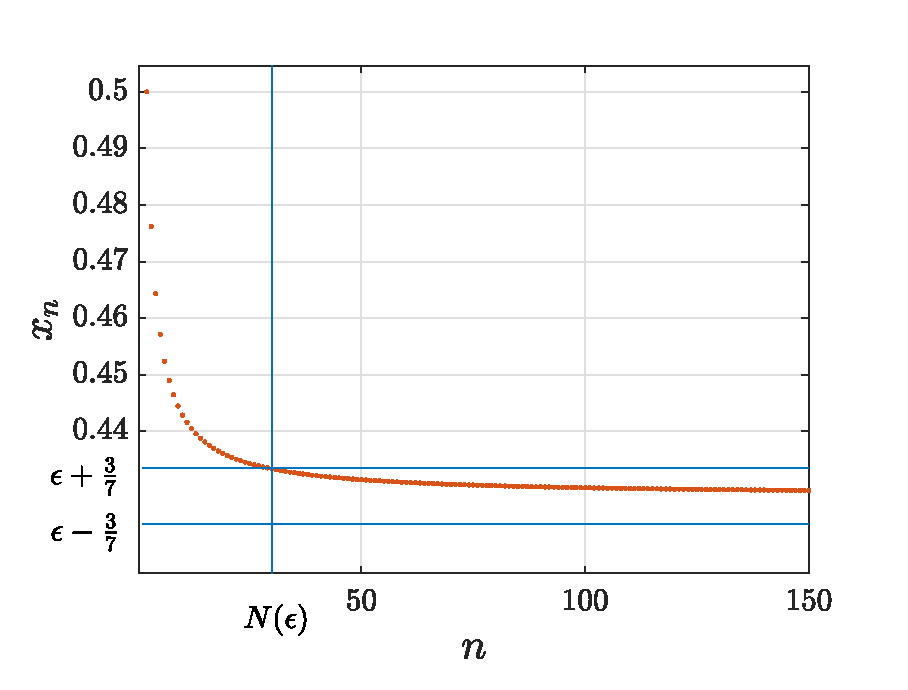
\includegraphics[width=0.75\textwidth]{convergence.eps}
        \caption{Notion de limite pour la suite $x_n=\frac{3n+1}{7n}$.}
        \label{fig:conv}
    \end{figure}\\ Nous illustrons ces remarques dans l'exemple suivant.

\subsection{Exemple - Limite d'une suite }
Soit la suite $x_n=\dfrac{3n+1}{7n}$. On peut réécrire $x_n = \dfrac{3}{7} + \dfrac{1}{7n}$. Comme $\frac{1}{n}$ (et a fortiori $\frac{1}{7n}$) devient très petit pour de grandes valeurs de $n$ (c'est-à-dire que $1/n \to 0$ lorsque $n\to \infty$), il semble raisonnable de conclure que $\lim\limits_{n\to \infty}{x_n}=\frac{3}{7}$. \\
En fait, ce raisonnement sera tout à fait valable après avoir introduit quelques autres propriétés, ce qui permettra d'écrire que 
\begin{equation*}
    \lim\limits_{n\to \infty}{x_n}=\lim\limits_{n\to \infty}{ \left[ \dfrac{3}{7} + \dfrac{1}{7n} \right] }= \dfrac{3}{7} + \lim\limits_{n \to \infty}{\left[ \dfrac{1}{7n} \right]} = \dfrac{3}{7} + \dfrac{1}{7} \cdot \lim\limits_{n \to \infty}{\left[ \dfrac{1}{n} \right] } = \dfrac{3}{7} + 0 = \dfrac{3}{7}. 
\end{equation*}
Analysons exactement ce que nous entendons par $\lim\limits_{n\to \infty}{x_n}=\frac{3}{7}$. 
\begin{center}

\begin{minipage}{0.75\textwidth}
  Par la définition \textcolor{blue}{\ref{definition_suite_convergence}}, $\lim\limits_{n\to \infty}{x_n}=\frac{3}{7}$ signifie que pour chaque $\epsilon>0$ il existe un nombre $N$ tel que
  \begin{equation}
      n>N \Longrightarrow \bigg|\displaystyle\frac{3n+1}{7n}-\frac{3}{7}\bigg|<\epsilon.
      %\label{eq_def_conv}
  \end{equation}
\end{minipage}
\end{center}
  Comme $\epsilon$ varie, $N=N_\epsilon$ varie. 
  \paragraph{Démonstration.}
Prouvons que $\lim\limits_{n \to \infty}{\displaystyle\frac{3n+1}{7n}}=\frac{3}{7}$. 
  \paragraph{}
  \textbf{1) Recherche de la condition sur $N$}. Il faut que pour tout $\epsilon>0$, on décide à quel point $n$ doit être suffisamment grand pour garantir $\bigg|\displaystyle\frac{3n+1}{7n}-\frac{3}{7}\bigg|<\epsilon$. Cela se réécrit
  \begin{equation*}
      \bigg|\displaystyle\frac{3n + 1}{7n} - \displaystyle\frac{3n}{7n}\bigg|<\epsilon \ \text{ ou encore } \ \bigg|\displaystyle\frac{1}{7n}\bigg|<\epsilon
  \end{equation*}
 La valeur absolue est ici redondante car $n \geq 0$. On peut donc isoler $n$:
  \begin{equation*}
      \bigg|\displaystyle\frac{1}{7n}\bigg|<\epsilon \iff \dfrac{1}{n} < 7 \epsilon \iff \dfrac{1}{7 \epsilon} < n.
  \end{equation*}
  Toutes les démarches que nous avons faites sont non seulement réversibles mais vraies pour tout $\epsilon>0$. Donc il suffit de poser  $N\geq \displaystyle\frac{1}{7 \epsilon}$ pour que \textcolor{blue}{$\eqref{eq_def_conv}$} soit vérifiée.
  \paragraph{}
  \textbf{2) Preuve formelle.}\\
  Soit $\epsilon>0$. On définit $N := \displaystyle\frac{1}{7 \epsilon}$. Alors pour $n>N$ : $$ \left| \dfrac{1}{7n} \right| = \left| \displaystyle\frac{3n + 1}{7n} - \displaystyle\frac{3}{7} \right| < \epsilon$$
Ainsi, pour tout $\epsilon > 0$, il existe un $N_\epsilon > 0$ tel que $$n > N_\epsilon \implies \left| x_n - \dfrac{3}{7} \right| < \epsilon.$$ 
Cela vérifie la définition donnée en \ref{definition_suite_convergence}, et donc $x_n$ converge bien vers $\frac{3}{7}$.
%En utilisant cette observation, nous trouvons que pour $\epsilon$ égal à $1, 0.1, 0.01$, et $0.001$ respectivement, $N$ peut être considéré comme approximativement $0.96, 4.45, 39.35$, et $388.33$ respectivement. Puisque nous ne nous intéressons qu'aux valeurs entières de $n$, (car $n\in \mathbb{N}$) nous pouvons tout aussi bien laisser tomber la partie fractionnaire de $N$. \paragraph{} Nous voyons alors que pour ces valeurs particulières de $N$, la relation \textcolor{blue}{$\eqref{eq_def_conv}$} donne
%\begin{equation*}
 %   \begin{aligned}
  %  n>0 & \text{ implique } \bigg|\displaystyle\frac{3n+1}{7n-4}- \displaystyle\frac{3}{7}\bigg|<1, \\
  %  n>4 & \text{ implique } \bigg|\displaystyle\frac{3n+1}{7n-4}- \displaystyle\frac{3}{7}\bigg|<0.1, \\
  %  n>39 & \text{ implique } \bigg|\displaystyle\frac{3n+1}{7n-4}- \displaystyle\frac{3}{7}\bigg|<0.01, \\
  %  n>388 & \text{ implique } \bigg|\displaystyle\frac{3n+1}{7n-4}- \displaystyle\frac{3}{7}\bigg|<0.001.
    %\end{aligned}
%\end{equation*}
\subsection{Unicité de la limite}
Il est assez facile de se convaincre que si $\lim x_n = x$ et $\lim x_n=y$, alors nous avons obligatoirement $x=y$. Les valeurs $x_n$ ne peuvent pas se rapprocher arbitrairement de valeurs différentes : si elles convergent, elles convergent vers un unique réel. \\
Pour le prouver, considérons $\epsilon >0$. Par la définition de la limite 
\textcolor{blue}{\eqref{eq_def_conv}}, il existe $N_1$ et $N_2$ tels que
\begin{align*}
    &\text{a) } \; n>N_1 \implies |x_n-x|<\displaystyle\frac{\epsilon}{2}. \\
    &\text{b) } \; n>N_2 \implies |x_n-y|<\displaystyle\frac{\epsilon}{2}.
\end{align*}
Dans la définition de convergence, la propriété est vérifiée \textit{pour tout} $\epsilon$. Ici, à partir d'\textit{un} $\epsilon$ arbitraire, on veut montrer une nouvelle propriété. On utilise alors les hypothèses initiales pour \textit{la} valeur $\frac{\epsilon}{2}$ plutôt que $\epsilon$, parce que l'étape suivante est:
$$\text{Pour } n>N_1, N_2, \text{ par l'inégalité triangulaire \textcolor{blue}{\eqref{inegal_tri}}, }$$
$$|x-y|=|(x-x_n)+(x_n-y)| \leq |x-x_n|+|x_n-y|\leq \displaystyle\frac{\epsilon}{2} +  \displaystyle\frac{\epsilon}{2} = \epsilon.$$
Ceci montre que $|x-y|<\epsilon$ pour tout $\epsilon>0$, ce qui force $|x-y|=0$, et ainsi $x=y$. \begin{flushright}
$\square$
\end{flushright}
Notons que ce choix d'appliquer la définition à $\frac{\epsilon}{2}$ pour obtenir $\epsilon$ en fin d'argument est purement esthétique. En effet, pour n'importe quel $\lambda > 0$, la propriété
$$\text{"Pour tout } \epsilon > 0 \text { il existe un } N_\epsilon \text{ tel que } n > N_\epsilon \implies |x_n-x| < \lambda \cdot \epsilon \text{."}$$
est rigoureusement équivalente à la propriété de convergence définie en \textcolor{blue}{\eqref{eq_def_conv}}. La conclusion aurait été parfaitement valide avec la valeur $2\epsilon$.
\section{Premiers Théorèmes}

Nous présentons ici les premiers résultats importants sur la convergence des suites réelles. \\
\\
\textbf{Théorème (Propriétés de la limite).} Soient $(x_n)$ et $(y_n)$ de limites $x$ et $y$ respectivement. Alors:
\begin{enumerate}
\item $\lim\limits_{n \to \infty} [ x_n + y_n ] = x + y$.
\item $\lim\limits_{n \to \infty} [ x_n \cdot y_n ] = x \cdot y$.
\item $\lim\limits_{n \to \infty} |x_n| = |x|$.
\end{enumerate}
\textit{Démonstration.} On prouve ici les propriétés (1.) et (3.), la propriété (2.) est laissée comme exercice. \\ \\
(1.) \\
Soit $\epsilon > 0$. Nous savons qu'il existe
\begin{align*}
&\text{a) } N_1(\epsilon) > 0 \text{ tel que } n > N_1 \implies |x_n - x| < \dfrac{\epsilon}{2}. \\
&\text{b) } N_2(\epsilon) > 0 \text{ tel que } n > N_2 \implies |y_n - y| < \dfrac{\epsilon}{2}.
\end{align*}
On déduit de a) et b) que $$n > N_1(\epsilon),N_2(\epsilon) \implies |x_n-x|+|y_n-y| < \epsilon.$$
À présent, grâce à l'inégalité triangulaire $|(x_n+y_n)-(x+y)| = |x_n-x+y_n-y| \leq |x_n-x|+|y_n-y|$, on sait que $$n > N_1(\epsilon),N_2(\epsilon) \implies |(x_n+y_n) -(x+y)| < \epsilon.$$
En prenant par exemple $N_\epsilon := N_1(\epsilon) + N_2(\epsilon)$, on a vérifié que
$$\text{Pour tout } \epsilon > 0, \text{ il existe un } N_\epsilon > 0 \text{ tel que } \; n > N_\epsilon \implies |(x_n+y_n) -(x+y)| < \epsilon,$$
c'est-à-dire que $\lim\limits_{n \to \infty} [ x_n + y_n ] = x + y$. \\
\\
\\
(3.) \\
Soit $\epsilon > 0$. Nous savons qu'il existe
$$N_\epsilon > 0 \text{ tel que } n > N_\epsilon \implies |x_n - x| < \epsilon.$$
L'inégalité triangulaire inverse $\Big| |x_n| - |x| \Big| \leq |x_n-x|$ nous permet immédiatement de conclure que
$$n > N_\epsilon \implies \Big| |x_n| - |x| \Big| < \epsilon,$$
et donc que $\lim\limits_{n \to \infty} |x_n| = |x|$.
\begin{flushright}
$\square$
\end{flushright}
\textbf{Théorème (des Gendarmes).} Soient $x_n$ et $z_n$ deux suites qui convergent vers la même limite $L$. \\
Si $x_n \leq y_n \leq z_n$ est vérifiée à partir d'un indice/rang $m \in \mathbb{N}$, alors $y_n$ converge vers $L$. \\ \\
\textit{Démonstration.} \\
Explicitons nos hypothèses:
\begin{align*}
    1)& \; \forall \epsilon > 0, \; \exists N_1(\epsilon) > 0 \text{ tel que } \; n \geq N_1 \implies \left| x_n - L \right| < \epsilon \\
    2)& \; \forall \epsilon > 0, \; \exists N_2(\epsilon) > 0 \text{ tel que } \; n \geq N_2 \implies \left| z_n - L \right| < \epsilon \\
\end{align*}
Soit donc $\epsilon > 0$: on veut trouver $N_3$ tel que $n > N_3 \implies \left| y_n - L \right| < \epsilon$. \\ \\
Si $N_3$ est plus grand que $N_1(\epsilon)$ et $N_2(\epsilon)$, soit $n > N_3$. \\
Grâce aux hypothèses 1) et 2), on sait que $L - \epsilon < x_n$ et $z_n < L + \epsilon$. \\
En supposant de plus que $N_3 > m$, pour que l'hypothèse $x_n \leq y_n \leq z_n$ soit valable, on obtient $$L-\epsilon < y_n < L + \epsilon,$$
ce qui est équivalent à $$ \left| y_n - L \right| < \epsilon.$$
Ainsi, en prenant $N_3$ plus grand que $m$, $N_1(\epsilon)$ et $N_2(\epsilon)$ (par exemple $N_3 = m + N_1(\epsilon)+ N_2(\epsilon)$), on a montré que pour tout $\epsilon > 0$, il existe un $N_3$ tel que $$n > N_3 \implies \left| y_n - L \right| < \epsilon,$$
et donc que $y_n$ converge vers $L$. \begin{flushright} $\square$
\end{flushright}
\vspace{1em}
\fbox{
\begin{minipage}{\textwidth}
  

\textbf{Théorème.} \begin{center}Toute suite bornée croissante (respectivement décroissante) converge vers son supremum (resp. infimum).\end{center}
\end{minipage}} \\
\\
\textit{Démonstration.} \\
Soit $(x_n)_{n \in \mathbb{N}}$ une suite croissante bornée, et $\alpha \in \mathbb{R}$ son supremum. \\
Soit $\epsilon > 0$: on veut montrer qu'il existe $N_\epsilon > 0$ tel que $n > N_\epsilon \implies | x_n - \alpha | < \epsilon.$ \\ \\
Par définition du supremum, on sait qu'il existe un élément $x_N \in \{ x_n : n \in \mathbb{N} \}$ tel que $$\alpha - \epsilon < x_N \leq \alpha.$$
La suite étant croissante, si $n > N$, on a $$\alpha - \epsilon < x_N \leq x_n \leq \alpha, \text{ c'est-à-dire } | x_n - \alpha | < \epsilon.$$
L'indice $N$ apparaissant dans la définition du supremum est donc suffisant: en prenant $N = N_\epsilon$ on a vérifié la définition de convergence. \\
Dans le cas décroissant, la preuve est analogue.
\begin{flushright}
$\square$
\end{flushright}
\textbf{Théorème (Critère de D'Alembert).} Soit $(x_n)_{n \in \mathbb{N}}$ une suite (qui ne vaut jamais 0). Supposons que la suite $$y_n := \left| \dfrac{x_{n+1}}{x_n} \right|$$
converge vers un réel $\rho \in \mathbb{R}$. \\
Alors: \\
$\bullet$ Si $\rho < 1$, $x_n$ converge vers 0. \\
$\bullet$ Si $\rho > 1$, $x_n$ diverge (et tend vers $+\infty$). \\
\\
La démonstration de ce théorème sera vue pendant le semestre. \\
\\
Notons que dans le cas $\rho = 1$, on ne peut pas conclure. La suite $x_n = n$ admet $\rho = 1$ et tend vers $+\infty$, la suite $y_n = \frac{1}{n}$ admet $\rho = 1$ et converge vers 0, la suite $z_n = (-1)^n$ admet $\rho = 1$ et oscille entre deux valeurs, etc.

\section{Sous-suites}
À partir de la notion de suite se définit naturellement la notion de sous-suite. Si $(x_n)_{n \in \mathbb{N}}$ est une suite réelle, on peut lui "enlever" des indices pour en définir une sous-suite. Tant qu'il reste un nombre infini d'indices, on a bien défini une nouvelle suite. \\ \\
Par exemple, on peut définir la sous-suite $(x_0,x_2,x_4,...)$ qui garde seulement les indices pairs, $(x_1,x_3,x_5,...)$ qui garde seulement les indices impairs, ou $(x_2,x_3,x_5,x_7,...)$ qui garde seulement les indices premiers. \\
Formellement, une sous-suite $y_k$ d'une suite $x_n$ est définie par l'application $f: \mathbb{N} \longrightarrow \mathbb{N}$ telle que $$y_k = x_{f(k)}.$$ Pour que cette définition soit correcte, il faut que $f$ soit strictement croissante. Souvent, on notera cette fonction $n_k$ : on dira que $x_{n_k}$ ou encore $(x_n)_{k\in \mathbb{N}}$ est une sous-suite de $x_n$. \\ \\
L'importance de la notion de sous-suite provient des deux théorèmes suivants, qui seront vus en cours durant le semestre. \paragraph{Théorème - Bolzano-Weierstrass.}
\paragraph{}
\fbox{
\begin{minipage}{\textwidth}
  \begin{center}
 Toute suite bornée admet une sous-suite convergente. Plus généralement, $E \subset \mathbb{R}$ est un ensemble borné si et seulement si toute suite dans $E$ admet une sous-suite convergente.
\end{center}
\end{minipage}}\\
\paragraph{}
\textbf{Théorème.} Une suite $(x_n)_{n \in \mathbb{N}}$ converge vers $L \in \mathbb{R}$ si et seulement si toutes ses sous-suites convergent vers $L$. \\
\\
Ce dernier théorème est particulièrement utile pour montrer qu'une suite n'est pas convergente: il suffit de trouver deux sous-suites qui convergent vers des valeurs différentes, ou une sous-suite qui ne converge pas.
\section{Suites de Cauchy}
La définition de la convergence d'une suite en \eqref{eq_def_conv} formalise l'idée intuitive de rapprochement \textit{vers une valeur fixe}. La définition de \textit{suite de Cauchy} utilise le même langage pour définir l'idée de rapprochement des valeurs de la suite \textit{entre elles}. \\
\\
\textbf{Définition.} Une suite $x_n$ est une suite de Cauchy si elle vérifie la propriété suivante.
\begin{center}
\fbox{
\begin{minipage}{0.75\textwidth}
  Pour tout $\epsilon>0$ il existe un nombre $N_\epsilon > 0$ tel que 
  \begin{equation}
      n,m > N_\epsilon \implies \big|x_n-x_m|<\epsilon.
      \label{eq_def_cauchy}
  \end{equation}
\end{minipage}
}
\end{center}
La force et l'importance de cette définition est qu'elle est équivalente à celle de suite convergente. L'une des implications de cette équivalence sera montrée en exercices, l'autre sera abordée pendant le semestre.
\section{lim sup et lim inf}
Les notions de \textit{limite supérieure} et \textit{limite inférieure} d'une suite sont importantes car elles sont bien définies pour toute suite bornée. \\
\\
Pour $x_n$ une suite bornée, définissons
$$y_n = \sup \{ x_k : k \geq n \}.$$
Pour un $n$ donné, $y_n$ prend donc comme valeur le supremum des "valeurs restantes" de $x_n$. \\
L'importance de cette suite est qu'elle est toujours \textit{décroissante}. Si $x_n$ est minorée, alors la suite $y_n$ converge vers une valeur que l'on définit comme la \textit{limite supérieure} de $x_n$:
$$\lim\limits_{n \to \infty} y_n =: \lim \sup x_n.$$
De la même manière, on peut définir la suite
$$z_n = \inf \{ x_k : k \geq n \}$$
qui est elle \textit{croissante} et, si $x_n$ est majorée, converge vers la \textit{limite inférieure} de $x_n$:
$$\lim\limits_{n \to \infty} z_n =: \lim \inf x_n.$$
À partir de ces notions, on a le résultat suivant. \\ \\
\textbf{Théorème.} Une suite $(x_n)_{n \in \mathbb{N}}$ converge vers $L \in \mathbb{R}$ si et seulement si
$$\lim \sup x_n = \lim \inf x_n = L.$$
%===============================
%===============================
%===============================
%===============================
%===============================%===============================

\chapter{Sommes Et Séries}
    Lors de calculs en analyse, des sommes de tout types apparaissent: il est donc utile de se familiariser avec. Ceci veut dire de calculer leur valeur pour des sommes simples, mais aussi savoir ce que l'on a le droit de faire et ne pas faire avec.
    
    Dans ce chapitre, nous introduisons d'abord les différences entre sommes finies et infinies, avant de calculer les valeurs de certaines sommes caractéristiques.
    
    Ceci à pour but de vous donner les bases nécessaires pour mieux comprendre le chapitre sur les \textit{séries} que vous étudierez pendant le semestre.
    \section{C'est quoi une somme en maths ?}
    En mathématiques, une somme est exactement ce que l'on entend par somme dans la vie de tout les jours. C'est l'addition répétée de différents termes.
    
    Par contre, vu qu'en maths on aime bien faire preuve de généralité et concision, au lieu de spécifier la valeur de chaque terme de la somme considérée, on l'exprime de manière plus compacte. On le fait en spécifiant la forme du terme général à sommer $x_n$, et des indices de départ et d'arrivée de la somme.
    
    Pour écrire la somme
    \[
        2+4+6+8+10+\dots+20,
    \]
    on utilisera alors plutôt l'écriture
    \[
        \sum_{k=1}^{10}2k.
    \]
    C'est tout de même bien pratique.
\section{Propriétés Des Sommes}
    En analyse on distingue d'un côté les sommes fines, caractérisées par un nombre de termes fini, et les sommes infinies, aussi appelés séries, qui sont composées d'une infinités de termes.
    
    Deux propriétés fondamentales sont cependant vraies pour les deux types de sommes.
    \begin{align*}
1)& \; \sum_{k=0}^{n}\lambda x_k=\lambda \cdot  \sum_{k=0}^{n}x_k \text{ pour tout } \lambda\in\mathbb{R}. \\
2)& \; \text{Si } y_k \geq x_k \text{ pour tout } k \in \{1,...,n\}, \text{ alors on a } \sum_{k=0}^{n}y_k \geq \sum_{k=0}^{n} x_k
    \end{align*}
    \subsection{Sommes finies}
        Il n'y a pas grand chose à dire sur les sommes finies à part que tout se passe comme on pourrait s'y attendre. Pour de telles sommes on a par exemple que  :
        \begin{center}
            \begin{minipage}{0.65\textwidth}
            \begin{enumerate}
                \item Le résultat est toujours fini.
                \item Réarranger l'ordre des termes ne change pas le résultat.
                \item La limite de la somme vaut la somme des limites.
            \end{enumerate}
            \end{minipage}
        \end{center}
    \subsection{Sommes infinies}
        Pour les sommes infinies, les résultats énoncés ci-dessus ne tiennent plus de manière générale. On peut alors résumer l'étude des sommes en analyse à la recherche de conditions sous lesquelles on peut procéder de la même manières que pour des sommes finies.
        
       % La première question que l'on peut se poser quand on considère des sommes infinie est ´´comment peut on écrire de telles sommes si elles ont une infinité de termes?''. La réponse est que l'on fourni le terme général de la suite des termes à sommer. Voyons ça de manière rigoureuse.
    \subsubsection{Définition.}
        Soit $(x_n)_{n\in\mathbb{N}}$ une suite réelle, on définit alors la \textit{suite des sommes partielles} associée $(S_n)_{n\in\mathbb{N}}$ par 
        \[
            S_n=\sum_{k=0}^{n}x_k,
        \]
        et la somme infinie, ou la \textit{série} associée à $(x_n)_{n\in\mathbb{N}}$ par 
        \[
            \lim_{n\to\infty}S_n=\sum_{k=0}^{\infty}x_k.
        \]
Les sommes infinies sont donc rigoureusement définies comme des limites de sommes finies. C'est pourquoi certaines sommes infinies sont dites valoir $+ \infty$ ou ne pas exister: certaines ne convergent pas vers un nombre réel. \\ \\
\textbf{Définition.}
        Lorsqu'une suite de sommes partielles a une valeur finie à la limite $n\to\infty$, i.e.
        \[
            \exists s\in\mathbb{R}\ t.q. \ \sum_{k=0}^{\infty}x_k=s,
        \]
         on dit que la série est \textit{convergente}. On dit alors de plus que la série associée vaut la valeur de la limite. \\
        Dans le cas contraire on dit que la série est \textit{divergente}.
    \subsection{Remarque}
        À première vue il peut paraître bizarre qu'une somme infinie de termes strictement positifs puisse converger. En réalité, si le terme général de la suite dont on considère la série décroît suffisamment vite, la  série est convergente. 
        
        Pour lever tout doute potentiel, considérons la suite sympathique de terme général $x_n=(1/2)^n$. La série qui lui est associée s'écrit alors par définition $\sum_{k=0}^{\infty}x_k=\sum_{k=0}^{\infty}(1/2)^n$. On a alors que le calcul de cette série est équivalent au calcul de la surface d'un rectangle $1\times 2$. Effectivement, chaque terme de la somme peut être associé à une partie de la surface du rectangle. La figure \ref{fig:somme_exemple} donne une représentation graphique de la solution. On en déduit que cette somme composée d'une infinité de termes admet une valeur finie, et vaut $\sum_{k=0}^{\infty}(1/2)^n=2$.
        \begin{figure}[h!]
            \centering
          
            \def\svgwidth{0.5\textwidth}
            \input{geometric_sum.pdf_tex}
            \caption{Représentation graphique des premières 4 contributions à la série $\sum_{k=0}^{\infty}(1/2)^k$. On peut se convaincre de la convergence de la série en remarquant qu'à la limite $n\to\infty$ la partie en blanc du rectangle sera tout juste complètement remplie. On en déduit donc que la série converge vers la surface du rectangle, donc 2.}
              \label{fig:somme_exemple}
        \end{figure}
\section{Sommes Arithmétiques Et Géométriques}
    Deux types de sommes dont il est important de savoir déterminer les valeurs sont celles associées à une suite arithmétique, i.e. une suite du type $x_n=x_0+nr$ pour un $r\in\mathbb{R_+}$, et celles associées à une suite géométrique, i.e. $x_n=x_0q^n$ pour un $q\in\mathbb{R}$. Dans cette section on se propose de déterminer la valeur de ces sommes.
    \subsection{Somme arithmétique}
        On considère la somme $S_n=\sum_{k=0}^{n}x_0+kr$, c'est à dire 
        \[
            S_n=x_0 + (x_0+r) + \dots + [x_0+(n-1)r]+ (x_0+nr).
        \]
        Pour expliciter sa valeur nous allons utiliser le fait que la somme du $k$-ième et du $(n-k)$-ième terme de $S_n$ est constante et vaut 
        \[
            x_{0+k}+x_{n-k}=(1+1)x_0 + (k+n-k)r = 2x_0+nr.
        \]
        
        En considérant d'abord le cas où $n$ est impair (donc le nombre de termes est pair) on trouve  
        \[
            S_n=\sum_{k=0}^{n}x_k=\sum_{k=0}^{(n-1)/2}x_{0+k}+x_{n-k}=\sum_{k=0}^{(n-1)/2}2x_0+nr=\frac{n+1}{2}(2x_0+nr),
        \]
        vu qu'il est possible de composer $(n-1)/2+1=(n+1)/2$ paires dont la somme vaut $2x_0+nr$.
        
        Considérons maintenant $n$ pair (donc le nombre de termes est impair). Dans ce cas $n-1$ est impair, et donc on a par ce qui a été vu précédemment 
        \[
            S_n=S_{n-1}+x_n=\frac{n}{2}[2x_0+(n-1)r] + x_0+nr=(n+1)x_0+\frac{n(n+1)}{2}r=\frac{n+1}{2}(2x_0+nr),
        \]
        qui est la même formule trouvée pour $n$ impair. Ceci est cohérent car pour $n$ pair on aurait pu commencer a sommer les $n/2$ paires $(x_0,x_n), ..., (x_{n/2-1},x_{n/2+1})$, et ensuite rajouter le terme $x_{n/2}$
        \[
            S_n=\frac{n}{2}(2x_0+nr) + x_0+\frac{n}{2}r=(n+1)x_0+\frac{n(n+1)}{2}r=\frac{n+1}{2}(2x_0+nr).
        \]
        On peut à présent réaliser notre rêve d'enfance et calculer la valeur de la somme des entiers compris entre 11 et 287 en posant $x_0=11,r=1,n=276$. Le résultat est $S=\frac{277}{2}(22+276)=41273$.
    \subsection{Somme géométrique}
        On considère la suite de sommes partielle de terme général $S_n=\sum_{k=0}^{n}x_0q^k$ avec $q>0$, c'est à dire
        \[
            S_n=x_0 + x_0r + \dots + x_0r^{n-1}+ x_0r^n.
        \]
        On a alors pour $q\ne 1$
        \[
            S_n - qS_n = \sum_{k=0}^{n}x_0q^k - \sum_{k=0}^{n}x_0q^{k+1} = x_0(1-q^{n+1})\implies S_n=x_0\frac{1-q^{n+1}}{1-q}.
        \]
        On en déduit en passant à la limite $n\to\infty$ que
        \[
            \sum_{k=1}^{\infty}x_0q^n = \begin{cases}\displaystyle  \frac{x_0}{1-q}, & q<1 \\
                \infty, & q\ge 1
                \end{cases},
        \]
        vue que d'autre part pour $q=1$ on a $S_n=(n+1)x_0\to\infty\ (n\to\infty)$.
        
        Notez que pour $q=1/2$ et $x_0=1$ on retrouve bien le résultat $\sum_{k=0}^{\infty}(1/2)^k=2$.
\section{Démonstration Par Récurrence Sur Les Sommes}

La démonstration par \textit{récurrence} (ou \textit{induction}) est, sous sa forme la plus simple, un type de preuve qui permet de prouver qu'une propriété $P(n)$ est vraie pour tous les entiers $n \in \{n_0, n_0 + 1, n_0 + 2, ...\}$ de la manière suivante

\begin{enumerate}
    \item \textbf{Initialisation} : Prouver $P(n_0)$
    \item \textbf{Hérédité} : Prouver que $P(n)$ implique $P(n+1)$ pour tout $n \geq n_0$
\end{enumerate}

En d'autres termes, l'étape d'initialisation prouve que la propriété $P$ est vraie pour le premier entier $n_0$ (en général, $n_0 = 0$ ou $1$) et l'étape d'hérédité nous explique comment obtenir $P(n_0 + 1)$ à partir de $P(n_0)$, comment obtenir $P(n_0 + 2)$ à partir de $P(n_0 + 1)$ etc... sans devoir expliciter tous les indices.

Avec une preuve par induction, on peut par exemple prouver que $2^n > 2n$ pour tout $n \geq 3$ ou encore que $11^n - 6$ est divisible par $5$ pour tout $n \geq 1$. Dans cette section, on va utiliser ce type de preuve pour reprouver les formules

$$\sum_{k=0}^n q^k = \frac{1-q^{n+1}}{1-q}, \quad \sum_{k=0}^n k = \frac{n(n+1)}{2}$$

qui ont été observées précédemment. 

\subsection{Somme arithmétique}
On prouve par récurrence que 
$$\sum_{k=0}^n k = \frac{n(n+1)}{2} \quad \forall n \geq 0$$

\textbf{Initialisation} : Pour $n = 0$, il faut vérifier que  $\sum_{k=0}^0 k = 0 = \frac{0 \cdot (0+1)}{2}$, ce qui est vrai.

\textbf{Hérédité} : Supposons que la formule $\sum_{k=0}^n k = \frac{n(n+1)}{2}$ soit vraie pour $n \geq 0$. Il faut en déduire la même identité, mais lorsque $n$ est remplacé par $n+1$, c'est-à-dire $\sum_{k=0}^{n+1} k = \frac{[n+1]([n+1]+1)}{2}$. 

En partant du côté gauche, on observe

\begin{alignat*}{2}
    \sum_{k=0}^{n+1} k &= (n+1) + \sum_{k=0}^{n} k && \\
    &= (n+1) + \frac{n(n+1)}{2} && \text{(hypothèse de récurrence)} \\
    &= \frac{2(n+1) + n(n+1)}{2} && \\
    &= \frac{n^2 + 3n + 2}{2} = \frac{(n+1)(n+2)}{2} =  \frac{[n+1]([n+1]+1)}{2}
\end{alignat*}

ce qui conclut la preuve par récurrence de l'identité.

\subsection{Somme géométrique}

On prouve par récurrence que 
$$\sum_{k=0}^n q^k = \frac{1-q^{n+1}}{1-q} \quad \forall n \geq 0$$

lorsque $q \neq 1$.

\textbf{Initialisation} : Pour $n = 0$, il faut vérifier que  $\sum_{k=0}^0 q^k = q^0 = 1 = \frac{1-q}{1-q}$, ce qui est vrai.

\textbf{Hérédité} : Supposons que la formule $\sum_{k=0}^n q^k = \frac{1-q^{n+1}}{1-q}$ soit vraie pour $n \geq 0$. Il faut en déduire la même identité, mais lorsque $n$ est remplacé par $n+1$, c'est-à-dire $\sum_{k=0}^{n+1} q^k = \frac{1-q^{[n+1]+1}}{1-q}$. 

En partant du côté gauche, on observe

\begin{alignat*}{2}
    \sum_{k=0}^{n+1} q^k &= q^{n+1} + \sum_{k=0}^{n} q^k && \\
    &= q^{n+1} + \frac{1-q^{n+1}}{1-q} && \text{(hypothèse de récurrence)} \\
    &= \frac{q^{n+1}(1-q) + 1-q^{n+1}}{1-q} && \\
    &= \frac{1-q^{n+2}}{1-q} = \frac{1-q^{[n+1]+1}}{1-q} 
\end{alignat*}

ce qui conclut la preuve par récurrence de l'identité.

\subsection{Autres exemples d'identités}

Les identités suivantes peuvent aussi être prouvées par récurrence.

\begin{align*}
   \sum_{k=0}^n k^2 &= \frac{n(n+1)(2n+1)}{6} \\
\sum_{k=0}^n k^3 &= \frac{n^2(n+1)^2}{4} = \left( \sum_{k=0}^n k \right)^2 \\
\end{align*}

\section{Convergence de sommes infinies}
\subsection{Une question délicate}
Comme mentionné précédemment, les "sommes infinies" sont rigoureusement définies comme les limites des sommes finies associées. \\
La série
$$ 1 + \dfrac{1}{2} + \dfrac{1}{4} + \dfrac{1}{8} + \dfrac{1}{16} + \dfrac{1}{32} + \cdots = 2$$ \\
vue en remarque \textbf{3.2.3} est par exemple définie comme
$$\sum_{n=0}^{\infty} \left( \dfrac{1}{2} \right) ^n = \lim_{N \to \infty} \left[ \sum_{n=0}^N \left( \dfrac{1}{2} \right) ^n \right].$$ \\
Assigner une valeur à une somme infinie, et a fortiori en parler comme une quantité arithmétique, n'a donc de sens \textit{que lorsqu'elle converge vraiment vers un nombre réel}. \\
C'est pourquoi les sommes infinies sont particulièrement difficiles à étudier: sans l'hypothèse de leur convergence, on aboutit facilement à des contradictions. \\
\\ \\
Par exemple, considérons la suite $x_n = (-1)^n$, et la somme associée
$$X_N := \sum_{n=0}^N x_n = 1 - 1 + 1 - 1 + \cdots + (-1)^N.$$
Naturellement, $X_N$ prend la valeur 1 lorsque $N$ est pair, et la valeur 0 lorsque $N$ est impair: elle ne peut donc pas converger. \\
Si cependant on décide de traiter la somme à l'infini comme une somme finie, on aboutit aux résultats suivants:
\begin{align*}
&\lim\limits_{N \to \infty} X_N = 1 - 1 + 1 - 1 + \cdots = (1-1) + (1-1) + \cdots = 0 + 0 + \cdots \implies \lim\limits_{N \to \infty} X_N = 0. \\
&\lim\limits_{N \to \infty} X_N = 1 - (1-1+1-1+ \cdots) = 1 - \lim\limits_{N \to \infty} X_N \implies 2 \cdot \lim\limits_{N \to \infty} X_N = 1 \implies \lim\limits_{N \to \infty} X_N = \dfrac{1}{2}.
\end{align*}
Mais aucun de ces résultats n'est valable: on a manipulé l'expression "$1-1+1-1+ \cdots$" comme une somme à valeur réelle alors qu'elle n'en est pas une. Cet exemple montre que la propriété fondamentale d'associativité $(a+b)+c = a+(b+c)$ pour les sommes finies ne s'étend pas forcément aux sommes infinies. \\
\\
La question la plus importante est donc de déterminer quand une somme infinie converge. L'étude de la convergence des suites au chapitre précédent nous permet d'établir certains critères.
\subsection{Critères de convergence}
La notion la plus évidente à appliquer ici est celle de suite de Cauchy, équivalente à la notion de convergence. \\
\\
\textbf{Proposition.} Soit $x_n$ une suite réelle et $X_N = x_0 + \cdots + x_N$ la suite de ses sommes partielles. \\
$X_N$ converge si et seulement si elle est de Cauchy, c'est-à-dire:
$$\text{Pour tout } \epsilon > 0 \text{ il existe } N_\epsilon > 0 \text{ tel que } n \geq m > N_\epsilon \implies |x_m + x_{m+1} + \cdots + x_{n-1} + x_n| < \epsilon.$$
\pagebreak \\
En particulier, si $X_N$ est convergente, alors en vérifiant le critère pour $m =n$ on obtient
$$\text{Pour tout } \epsilon > 0 \text{ il existe } N_\epsilon > 0 \text{ tel que }n > N_\epsilon \implies |x_n| < \epsilon, \text{ et donc } \lim_{n \to \infty } x_n = 0.$$
Cet énoncé ne doit pas surprendre. Si la suite $x_n$
ne devenait pas "de plus en plus négligeable", la somme de ses termes ne pourrait pas se "stabiliser" vers une valeur fixe.
\\
\\
Notons que cette condition est loin d'être suffisante! Le contre-exemple le plus connu est celui de la suite $x_n = \frac{1}{n}$. \\
$x_n$ converge bien vers 0 mais $$\sum_{n=0}^{\infty} x_n = 1 + \dfrac{1}{2} + \dfrac{1}{3} + \dfrac{1}{4} + \dfrac{1}{5} + \cdots \longrightarrow +\infty.$$
La preuve de ce fait sera un exercice. \\ \\
\textbf{Proposition (Critères de comparaison).} Soient $x_n$ et $y_n$ deux suites vérifiant $0 \leq x_n \leq y_n$ pour tout $n$ et $X_N$, $Y_N$ leurs sommes partielles associées. \\
$\bullet$ Si $Y_N$ converge, alors $X_N$ converge également et $\lim\limits_{N \to \infty} X_N \leq \lim\limits_{N \to \infty} Y_N$. \\
$\bullet$ Si $X_N$ ne converge pas (et donc, dans ce cas, tend vers $+\infty$), alors $Y_N$ ne converge pas non plus. \\ \\
Ce critère permet de simplifier l'étude des sommes de signe constant : en inversant les signes, on obtient des conclusions analogues. \\
\\
\textbf{Théorème (Critère de D'Alembert, partie II).} Soit $x_n$ une suite réelle et $X_N$ sa somme partielle. Sous la même hypothèse que pour les suites, si $$y_n := \left| \dfrac{x_{n+1}}{x_n} \right|$$ converge vers un réel $\rho \in \R$, alors: \\
$\bullet$ Si $\rho < 1$, $X_N$ (et même $|X_N|$) converge. \\
$\bullet$ Si $\rho > 1$, $X_N$ diverge (et $|X_N|$ tend vers $+\infty)$. \\ \\
Notons qu'à nouveau, tout peut se produire si $\rho = 1$. C'est le cas pour $x_n = \frac{1}{n}$, dont la somme diverge, et pour $x_n = \frac{1}{n^2}$, dont la somme converge.
%===============================
%===============================
%===============================
%===============================
\chapter{Utilitaires}
\section{Binôme de Newton}
\label{binomenewt}

Si $x$ et $y$ sont deux éléments d'un \textbf{anneau}\footnote{En algèbre, un anneau est une structure algébrique fondamentale. C'est un ensemble sur lequel deux opérations satisfont certaines des propriétés de l'addition et la multiplication des nombres entiers relatifs. } qui \textbf{commutent} (c'est à dire tels que $xy=yx$), alors pour tout entier naturel $n$ , 
\boldmath{}

\begin{equation}
    (x+y)^{n}=\sum_{k=0}^{n}\binom{n}{k}x^ky^{n-k}=\sum_{k=0}^n\binom{n}{k}x^{n-k}y^k
\end{equation}
\unboldmath{} où $\binom{n}{k}=\displaystyle\frac{n!}{k!(n-k)!}$.
Pour démontrer la formule du binôme de Newton par récurrence il est utile de noter que : \ \begin{eqnarray}
\binom{n}{k}+\binom{n}{k-1}=\binom{n+1}{k}
\end{eqnarray}
\section{Inégalité triangulaire}\label{inegalite_triangulaire}

En géométrie, l'inégalité triangulaire est le fait que, dans un triangle quelconque, la longueur d'un côté est inférieure à la somme des longueurs des deux autres côtés. Dans la vie quotidienne, comme en géométrie euclidienne, elle se traduit par le fait que la ligne droite est le plus court chemin : le plus court chemin d'un point $a$ à un point $b$ est d'y aller tout droit, sans passer par un troisième point $c$ qui ne serait pas sur la ligne droite. 
\begin{equation}
|a+b|\leq |a|+|b|, \text{ pour tout } \ a,b.
    \label{inegal_tri}
\end{equation}
 \begin{figure}[!h]
     \centering
     \includegraphics[width=8cm]{Triangle.png}
     \caption{}
     \label{inegal_tri_geom}
 \end{figure}
\section{Fonctions particulières }\label{fonctionsparticulieres}
 \subsection{Partie entière }
 \subsubsection{Proposition} A tout nombre réel $x$, on peut associer un unique entier relatif $[x]$ tel que $$  [x]\leq x \leq [x]+1$$ ou encore $$ [x]-1<x \leq [x]$$
 $[x]$ est appelé la \textbf{partie entière } de $x$. Autrement dit, $[x]$ est le plus grand entier naturel relatif inférieur ou égal à $x$.
 \subsection{Exemple de limites}
 \begin{equation*}
     \begin{array}{c c l}
          \lim\limits_{x \to +\infty}{\displaystyle\frac{x}{1+[x]}}& \forall x\geq 1:\displaystyle\frac{[x]}{1+[x]}\leq \displaystyle\frac{x}{1+[x]}\leq \displaystyle\frac{x}{x}& \Longrightarrow \lim\limits_{x \to +\infty}{\displaystyle\frac{x}{1+[x]}}=1   \\
          \\
           \lim\limits_{x \to 0}{x[\displaystyle\frac{1}{x}]}& \forall x\in\mathbb{R}^* : \displaystyle\frac{1}{x}-1<[\displaystyle\frac{1}{x}]\leq \displaystyle\frac{1}{x}& \Longrightarrow \lim\limits_{x \to 0}{x[\displaystyle\frac{1}{x}]}=1
     \end{array}
 \end{equation*}
 \subsection{Fonction exponentielle}
 \subsubsection{Définition} Puisque tout $x\in \mathbb{R}$, la série $\displaystyle\sum_{n=0}^{+\infty}\displaystyle\frac{x^n}{n!}$ est absolument convergente (Critère de D'Alembert le prouve aisément), on pose, par définition : $$e^x=\displaystyle\sum_{n=0}^{+\infty}\frac{x^n}{n!} $$
 La fonction exp:$\mathbb{R}\to \mathbb{R}$ définie par $exp(x)=e^x$ est appelée fonction \textbf{exponentielle}. Elle est continue, strictement croissante et bijective.\\
 Par convention , $0^0=0!=1$
 \subsubsection{Propriétés}
 \begin{equation*}
     \begin{array}{l c }
          1)\text{ } \forall x\in \mathbb{R}: &  e^x>0
          \\
          \\
          2)
         &\lim\limits_{x\to -\infty}{e^x}=0 \text{ et }  \lim\limits_{x\to +\infty}{e^x}=+\infty
         \\
         3) & e^0=1 \text{ et } e^1=\displaystyle\sum_{n=0}^{+\infty}\frac{1}{n!}= e =\lim\limits_{n\to +\infty}{(1+\displaystyle\frac{1}{n})^n}\\
         4)\text{ } \forall x,y\in \mathbb{R}: & e^{x+y}=e^x.e^y
         \\
         \\
         5)\text{ } \forall x\in \mathbb{R}:& e^{-x}=\displaystyle\frac{1}{e^x}
         \\
         \\
         6)\text{ } \forall x\in \mathbb{R}_+^* \text{ et } k\in \mathbb{N}: & e^x>\displaystyle\frac{x^k}{k!} \text{ et } e^{-x}<\displaystyle\frac{k!}{x^k}\\
         \\
         7)\text{ } \forall x\in \mathbb{R}: & e^x=\lim\limits_{n\to + \infty}{(1+\frac{1}{n})^n}
     \end{array}
 \end{equation*}
 \subsection{Fonction Logarithme de base a}
 Soient a>0 et $a\neq 1$. La fonction notée $\log_a:\mathbb{R}_+^*\to \mathbb{R}$ et définie par $$\log_a{x}=\displaystyle
\frac{\ln{x}}{\ln{a}} $$
 \subsubsection{Propriétés}
 \begin{equation*}
     \begin{array}{l c}
     
        1)   & \log_a{1}=0 \text{ et } \log_a{a}=1.  \\
        \\
         2) \text{ Si } 0<a<1: & \lim\limits_{x\to 0^+}{\log_a{x}}=+\infty \text{ et } \lim\limits_{x\to +\infty}{\log_a{x}}=-\infty\\
         \\
         3) \text{ Si } a>1 : & \lim\limits_{x\to 0^+}{\log_a{x}}=-\infty \text{ et } \lim\limits_{x\to +\infty}{\log_a{x}}=+\infty\\
         \\
         4) \forall x,y\in\mathbb{R}_+^* : & \log_a{xy}=\log_a{x}+\log_a{y} \text{ et } \log_a{\displaystyle\frac{x}{y}}=\log_a{x}-\log_a{y}
     \end{array}
 \end{equation*}
 \subsection{Fonction exponentielle de base a}
 \subsubsection{Définition} Soient $a>0$ et $a\neq 1$. La fonction $\log_a:\mathbb{R}_+^*\to \mathbb{R}$ étant bijective, elle admet une fonction réciproque, appelée fonction \textbf{exponentielle de base a } et notée $\exp_a$. Cette fonction $\exp_a:\mathbb{R}\to \mathbb{R}_+^*$ est continue, strictement croissante si $a>1$ et strictement décroissante si $0<a<1$. De plus, par définition, on pose : $$ a^x=\exp_a{(x)}$$.
 \subsubsection{Propriétés}
  $$  \begin{array}{l c }
          1) \forall x\in \mathbb{R} :& a^x=\exp_a{(x)}=e^{x\ \ln{(a)}}  \\ \\
          2) & a^0=1 \text{ et } a^1=a \\ \\
          3) \text{ Si } 0<a<1 : & \lim\limits_{x\to -\infty}{a^x}= +\infty \text{ et } \lim\limits_{x\to +\infty}{a^x}= 0 
          \\
          \\
          4)\text{ Si } a>1 :& \lim\limits_{x\to -\infty}{a^x}= 0 \text{ et } \lim\limits_{x\to +\infty}{a^x}= +\infty \\ 
          \\
          5) \forall x\in \mathbb{R} :& \ \ln{a^x}=x\ \ln{a} \text{ et } \log_a{a^x}=x 
          \end{array}$$
          

         $$ \begin{array}{l c }
          6) \forall x,y\in \mathbb{R} :& a^{x+y}=a^x.a^y \text{ et } (a^x)^y=a^{xy}\\ \\
          7) \forall x\in \mathbb{R} :& a^{-x}=\displaystyle\frac{1}{a^x}=(\displaystyle\frac{1}{a})^x \\
          \\
          8) \forall x\in \mathbb{R} :& (ab)^x=a^x.b^x \text{ et } (\displaystyle\frac{a}{b})^x=\displaystyle\frac{a^x}{b^x}
     \end{array} $$

 \begin{figure}[!h]
     \centering
     \includegraphics[width=10cm]{13CBF6C6-736D-45BC-B39D-BE32DC3C9F00.jpeg}
     \caption{Représentation graphique de la fonction $a^x$ pour différentes valeurs de $a$ (décroissante pour $a<1$). }
     \label{fonctionpuissance}
 \end{figure}
 
 \subsection{Fonction puissance }
 \subsubsection{Définition} Soit $\alpha$ un nombre réel fixé. La fonction $f: \mathbb{R}_+^*\to \mathbb{R}_+^*$ définie par  $$ f(x)=x^{\alpha}=e^{\alpha\\ln{x}},$$ est appelée fonction \textbf{puissance}. Cette fonction est continue, strictement croissante si $\alpha>0$, constante si $\alpha=0$ et strictement décroissante si $\alpha<0$
 \subsubsection{Propriétés}
 \begin{equation*}
     \begin{array}{l c}
          1) \text{ Si } \alpha<0: &  \lim\limits_{x\to 0^+}{x^{\alpha}}=+\infty \text{ et }  \lim\limits_{x\to +\infty}{x^{\alpha}}=0 \\ 
          \\
          2) \text{ Si } \alpha>0: &  \lim\limits_{x\to 0^+}{x^{\alpha}}=0 \text{ et }  \lim\limits_{x\to +\infty}{x^{\alpha}}=+\infty\\ \\
          3) \forall x\in \mathbb{R}_+^*:& \log_a{x^{\alpha}}=\alpha\log_a{x} \\
          \\
          4) \forall x\in \mathbb{R}_+^*: & x^{\alpha+\beta}=x^{\alpha}.x^{\beta} \text{ et } (x^{\alpha})^{\beta}=x^{\alpha\beta}\\ 
          \\ 
          5) \forall x,y\in \mathbb{R}_+^*: & (xy)^{\alpha}=x^{\alpha}y^{\alpha} \\ 
          \\ 
          6) \forall x,y\in \mathbb{R}_+^*: & (\displaystyle\frac{x}{y})^{\alpha}=\displaystyle\frac{x^{\alpha}}{y^{\alpha}} \\ 
          \\
          7) \text{ Si} 0<a<1 \text{ et } \alpha>0 :& \lim\limits_{x\to + \infty}{\displaystyle\frac{a^x}{x^{\alpha}}}=0 \\ 
          \\
          8) \text{ Si } a>1 :& \lim\limits_{x\to + \infty}{\displaystyle\frac{a^x}{x^{\alpha}}}=+\infty \\ 
          \\
          9) \forall \alpha >0 : & \lim\limits_{x\to +\infty}{\displaystyle\frac{\log_a{x}}{x^{\alpha}}}=0 \text{ et } \lim\limits_{x \to 0^+}{ x^{\alpha}\log_a{x}}=0
     \end{array}
 \end{equation*}
%==========================================================================
%==========================================================================
%==========================================================================
%==========================================================================%==========================================================================
%==========================================================================
%==========================================================================
%==========================================================================
%==========================================================================
%==========================================================================
%==========================================================================
%==========================================================================
%==========================================================================
%==========================================================================
%==========================================================================
%==========================================================================%==========================================================================
%==========================================================================
%==========================================================================
%==========================================================================
%==========================================================================
%==========================================================================
%==========================================================================
%==========================================================================
%==========================================================================
%==========================================================================
%==========================================================================
%==========================================================================%==========================================================================
%==========================================================================
%==========================================================================
%==========================================================================
%==========================================================================
%==========================================================================
%==========================================================================
%==========================================================================
%==========================================================================
%==========================================================================
%==========================================================================
%==========================================================================%==========================================================================
%==========================================================================
%==========================================================================
%==========================================================================

\end{document}